\chapter{Introduction} \label{ch:intro}

%% =====================================================================================
%%
%%              G E N E R A L  I N T R O D U C T I O N
%%
%% =====================================================================================

%% From Just
A pair of massive stars at the end of their evolution undergo \acp{SN} explosions, and 
if stars are sufficiently massive, a pair of compact objects orbiting each other is formed. 
One of the possible outcomes, is a pair of \acp{NS}, compact, but heavy objects sustained 
against gravitational collapse by the neutron degeneracy pressure. 
The theory of \ac{GR} predicts that the orbit of the system shrinks, as \acp{NS} loose energy 
and angular momentum to \acp{GW}. The stars inspiral until they collide at the last orbit. 
%ejecting a small fraction of matter into the Universe, leaving a \pmerg{} remnant.


The high compactness of \acp{NS} leads to an energetic, explosive merger, where a small 
fraction of the \ac{NS} matter is ejected from the system at mildly relativistic 
velocities. 
Additionally, the massive \pmerg{} remnant and sorrounding it gravitationally bound 
matter are subjected to complex dynamical interactions, weak processes and magnetically induced 
turbulence, that might induce additional matter outflows. This makes the \ac{BNS} mergers 
strong contributors to the cosmic chemical evolution. 
The matter ejected at/after mergers, \ie, ejecta, has unique properties, rarely found in other 
astrophysical sites. Specifically, the abundance of free neutrons allow for the so-called 
rapid neutron capture process (\rproc{}), 
The \rproc{}, that is responsible for the production of the heaviest elements in the 
Universe, lanthanides and actinides. 

%Mergers of \acp{BNS} are at the center of a variety of physical processes in astrophysics.
Wide range of possible types and properties of ejecta lead to a similarly broad 
range in \ac{EM} counterparts to \ac{BNS} mergers. For instance, the heavy elements 
produced via \rproc{} \nuc{} eventually decay, powering the quasi-thermal \ac{EM} 
counterpart, \ac{kN}. Additionally, it \ac{BNS} mergers are expected to produce 
powerful jets, that can be observed as \acp{SGRB}. Moreover, expanding into \ac{ISM} 
medium, \ac{BNS} merger ejecta is expected to generate non-thermal, long-lasting 
afterglow emission. 
%Perhaps, two of the most 
%well studied ones are the \ac{kN}, a thermal counterpart powered by the decay of 
%newly synthesized heavy elements in the ejecta, and \acp{SGRB}, generally non-thermal 
%emission from the ultrarelativistic collimated outflow, formed after the merger. 
Together with \ac{GW} emission, these signals allow to study the processes occuring 
at mergers to a great detains, origin of the \ac{SGRB}, cosmic chemical evolution, 
and, perhaps most importantly, they provide unique constraints on the theory of gravity 
and density of matter at many times the nuclear saturation densities. 
%Study of these \ac{EM} counterparts in conjuncture with \acp{GW} emission allows to 
%gain unique insigts into the inner workings of the \ac{BNS} merger and previously 
%unobtainable constraints on the theory of gravity, the properties of matter at 
%supranuclear densities, origin of the \ac{SGRB}, cosmic chemical evolution. 



In August 2017, the first \ac{BNS} merger was observed 
as a source of \ac{GW} waves by \ac{LIGO}/Virgo, \GW{}. The unprecedented \ac{EM} 
follow-up campaign, spanning hundreds of observatories across the world lead to 
the identification of the merger \ac{EM} counterparts: \ac{kN}, \AT{} and 
\ac{SGRB}, \GRB{} 
\citep{TheLIGOScientific:2017qsa,Abbott:2018wiz,GBM:2017lvd}. 
%
\acp{GW} shed light on the properties of cold matter 
at supernuclear densities, the \ac{NS} \ac{EOS} 
\citep{Hinderer:2009ca,Damour:2012yf,DelPozzo:2013ala}, while 
the properties of matter at densities several times that of the 
nuclear matter, as well as the astrophysical implications of the merger 
were largely derived from the \ac{EM} signals 
\cite{Alexander:2017aly,Villar:2017wcc,Hajela:2019mjy}. \red{add proper refs}


The complexity, non-linearity, non-stationarity and multidimensionality of physical 
processes operating at \ac{BNS} mergers on a wide range of scales of length and time 
implies that self-consistent, quantitative studies are only possible with numerical 
simulations 
\citep{Sekiguchi:2011zd,Wanajo:2014wha,Foucart:2015gaa,Palenzuela:2015dqa,Sekiguchi:2016bjd,Kiuchi:2017zzg,Radice:2017zta,Fujibayashi:2017puw,Radice:2018pdn}.
These simulations, performed with \ac{NR} codes that took years, sometimes 
decades to develop and test, are very computationally expensive, rare, and require detailed 
postprocessing and analysis. 
%
Moreover, the self-consistent modeling of the \ac{BNS} merger and its \ac{EM} counterparts 
is still beyond the reach of modern methods. Generally, the short-term (hundred of milliseconds) 
evolution of the merger itself is handled with \ac{NR} codes while the 
\nuc{} and \ac{EM} emission are computed after, in postprocessing. 
%Strengthening the connection between these methods is one of the goals of this thesis. 
%
%In the following sections we sketch the astrophysical background to clarify the 
%context of our study and we conclude the chapter by summarizing the main points of 
%motivation for this thesis and its structural arrangement.

In this thesis we postprocess a large set of \ac{NR} \ac{BNS} merger simulations, 
performed with the state-of-the-art \ac{NR} code, \wisky{}, and targeted to the 
\GW{} (with corresponding binary parameters).
%
We focus on the \pmerg{} matter dynamics and properties of ejecta. 
We asses the nucleosynthetic yields in the ejecta, placing them into astrophysical 
context. Using the \ac{kN} model, developed by \citet{Perego:2017wtu}, we analyze 
the \ac{EM} signatures of our \ac{BNS} merger models, comparing them with \AT{}. 
Additionally, we develop a new code to model non-thermal emission from ejecta 
expanding into \ac{ISM}, apply it to the outcome of the merger simulations and 
compare the results with recently observed change in \ac{SGRB} emission. 
%
The main goal of our study is to strengthen the link between the ab-inito 
numerical relativity simulations and observations of \ac{EM} signatures of mergers, 
and in doing so, provide better constraints on the properties of \GW{} 
and ultimately, on the properties of matter and supranuclear densities.



%Single \acp{NS} are very compact but massive objects, 
%%where compactness $C_{i} = GM_i/R_i^2c^2\propto0.15$ and 
%for description of which the effects of \ac{GR} cannot be neglected. 
%%
%A pair of \acp{NS} orbiting each other slowly loses its 
%angular momentum to \acp{GW}. 
%%The timescale for the radiation reaction, however, 
%%is much longer than the orbital period for most of the inspiral and the 
%%system evolution can be considered adiabatic. 
%%For instance, the inspiral can be considered as a sequence of circular orbits. 
%%However, during last orbits before merger, the finite size (tides) and \ac{HD}
%%effects starts to become important. 
%The inspiral ends at the onset of the Roche lobe overflow, when the binary 
%reaches the mass-shedding limit \citep{Bejger:2004zx}.
%
%%% <<< From Radice Review >>>
%Mergers of \acp{BNS} are at the center of a variety of physical processes 
%in astrophysics.
%The first ever detection of such event by \ac{LIGO}/Virgo, \GW{}, 
%followed up by detections across \ac{EM} spectrum 
%have significantly advanced our understanding 
%of gravity, physics of dense matter, origins of \acp{SGRB} and \rproc{} elements 
%\citep{TheLIGOScientific:2017qsa,Abbott:2018wiz,GBM:2017lvd}. 
%%
%Specifically, while \acp{GW} shed light on the properties of cold matter 
%at supernuclear densities, the \ac{NS} \ac{EOS} 
%\citep{Hinderer:2009ca,Damour:2012yf,DelPozzo:2013ala}, 
%the properties of matter at densities several times that of the 
%nuclear matter, as well as the astrophysical implications of the merger 
%were largely derived from the \ac{EM} signals. 
%
%%Emitted during the inspiral, \acp{GW} delivered a plethora of information about  
%%\ac{NS} \ac{EOS} at supernuclear densities 
%%\citep{Hinderer:2009ca,Damour:2012yf,DelPozzo:2013ala}. 
%%%
%%The properties of matter at densities several times that of the 
%%nuclear matter, however, were not well constrained, as the \pmerg{} \ac{GW} 
%%was not detected. Future observations of the high frequency \pmerg{} signal 
%%will shed more light on these properties 
%%\citep{Sekiguchi:2011mc,Radice:2017lry,Most:2018eaw,Bauswein:2018bma}, 
%%constraining one of the main quantities, the tidal deformability.
%
%The \ac{EM} signal originates from the matter ejected during or after 
%the merger by a variety of physical processes, the so-called, ejecta.
%%
%The conditions within ejecta, are such that the rapid neutron capture (\rproc{}) 
%\nuc{}, responsible for the production of the heaviest elements in the Universe
%such as gold can take place \citep{Cowan:2019pkx}.
%%
%Notably, whether \acp{BNS} mergers are the prime source of this material is still unknown.
%% This was confirmed by \ac{MM} observations of \GW{} \cite{12}. 
%% however, it is unclear whether \ac{BNS} mergers is the dominant source of 
%% \rproc{} elements in the universe, or if other \rproc{} cites are required to 
%% explain the observed abundances in the oldest stars, \ac{UFG} and our solar system. 
%
%
%
%In order to study the dynamical phase of \ac{BNS} mergers and \pmerg{} evolution, 
%sophisticated \ac{NR} simulations are required. Modern, state-of-the-art methods 
%include full \ac{GR}; composition-dependent nuclear \ac{EOS} with finite-temperature 
%effects, \ac{GRMHD} and advanced neutrino transport with varying degree of approximation,
%\citep{Sekiguchi:2011zd,Wanajo:2014wha,Foucart:2015gaa,Palenzuela:2015dqa,Sekiguchi:2016bjd,Kiuchi:2017zzg,Radice:2017zta,Fujibayashi:2017puw}.
%
%%In this thesis we perform \ac{NR} simulations of \ac{BNS} mergers, report on their 
%%qualitative and quantitative picture and its implication for the \ac{EM} signatures.
%%We focus on the nuclear astrophsyics aspect of the mergers, and on the comparison 
%%between theoretical predictions and observations of \GW{}, discussing the 
%%\rproc{} \nuc{}, thermal \ac{EM} transient, and non-thermal \ac{EM} afterglow. 


%% =====================================================================================
%%
%%              T H E O R E T I C A L  P I C 
%%
%% =====================================================================================

\section{Theoretical picture of \ac{BNS} mergers}

In this section we provide a brief summary of the current picture of the 
\ac{BNS} mergers, their impact on the galactic chemical evolution, and their 
\ac{EM} counterparts. For the sake of brevity we allude most of the technical details, 
and we refer the interested reader to the following reviews and references therein.
%
For the general overview on the topic we refer to \citet{Shibata:2016},
For a more recent reviews done by different leading groups we refer to 
\citet{Radice:2020ddv,Bernuzzi:2020tgt,Shibata:2019wef}.


\subsection{Inspiral}

The inspiral phase of the \ac{BNS} system is primarily governed by the emission 
of \acp{GW}. Several approximations exists to describe this phase.
When stars are sufficiently far apart, the \ac{PN} approximation to \ac{GR} 
(the expansion in $\upsilon/c$, with $\upsilon/c\ll 1$) can be used. 
%The dynamics of two stars, that are sufficiently separated to have relatively small 
%angular velocity can be described via the \ac{PN} approximation to \ac{GR} 
%(the expansion in $\upsilon/c$, with $\upsilon/c\ll 1$). 
%In reality, however, \acp{NS} are not point-masses. The finite size (tidal) effects 
%modify the inspiral and, consequently, emitted \acp{GW}. 
Another approximation to the two-body dynamics in \ac{GR} is the \ac{EOB} formalism,
which is a Hamiltonian formalism, applicable to all stages of the binary evolution.
%
The latter has the advantage for taking into account the finite size of \acp{NS}, \ie, 
how the gravitational field of one star affects another, so-called tidal effects. 
Their description involves the stars' dimensionless relativistic Love numbers \citep{Damour:2009vw,Binnington:2009bb}, which in the case of quasi-static 
external field can be computed by considering the stationary perturbations 
of the spherical relativistic star, \ie, solving the stellar structure, 
\ac{TOV} equations in full \ac{GR}.
% taking into account the strong dependency of the 
%tidal coefficients on the star compactness, defined as $C_{i} = GM_i/R_i^2c^2$. 
These, Love numbers carry the imprint of the \ac{EOS} on the \ac{BNS} dynamics.
%
The inclusion of tidal effects manifests as a faster inspiral and merger at higher 
frequency of \acp{GW} \citep{Damour:2009wj}.

For a \ac{BNS} system it is common to introduce the 
\textit{reduced tidal deformability} as 
%
\begin{equation}
\label{eq:intro:Lambda}
\tilde{\Lambda} = \frac{16}{13}\frac{(M_A + 12M_B)M_A^4}{M^5}\Lambda_A + (A\leftrightarrow B).
\end{equation}
%
where $\Lambda_2^i = 2/3 k_2^i (c^2 R_i/GM_i)^5$ with $i\in\{A,B\}$, 
$M_i$ is the gravitational mass,
and $M$ is the total gravitational mass of the system.
%
The effects of tides appear in \ac{GW} waveform calculations, as radiation reaction 
complimenting the conservative dynamics of the binary \citep{Damour:2008gu}. 
%(see also \citet{Damour:2012yf,Banihashemi:2018xfb}).


From the analysis of \acp{GW} \GW{} was interpreted as \ac{BNS} merger with total mass of
${\simeq}2.7\,\Msun$, chirp mass $\mathcal{M}=( (M_A M_B)^{3/5} / (M_A + M_B)^{1/5} ) = 1.186(1)\,\Msun$, \mr{} $q\in[1,1.34]$ 
and $\tilde{\Lambda}\simeq300$ (with an upper bound of ${\sim}800$)
\citep{TheLIGOScientific:2017qsa,Abbott:2018wiz,LIGOScientific:2018mvr}.
%Inclusion of the \ac{EM} counterparts into the analysis resulted in higher $\tilde{\Lambda}$ being 
%more favored \citep{Radice:2017lry,Radice:2018ozg,Breschi:2021tbm}.


\subsection{Merger and \pmerg{}}\label{sec:intro:merg_pmerg}

%% --------------------------------------------------------------------------
%%               P O S T - M E R G E R
%% --------------------------------------------------------------------------

\begin{figure}[t]
    \centering
    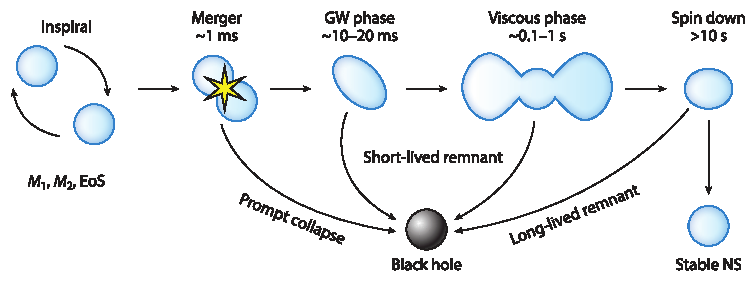
\includegraphics[width=0.70\textwidth]{Fig_3_Rad.pdf}
    \caption{
        Overview of the different phases in an \ac{NS} merger and the relative timescales. 
        The inspiral ends with the merger, when the two stars start to fuse together. 
        The early \pmerg{} evolution is entirely driven by hydrodynamics and by \ac{GW} emission. 
        If the remnant does not collapse within ${\sim}10-20\,$ms, \ac{GW} losses
        subside and other physical processes become more important: 
        Angular momentum redistribution (which is due to turbulent viscosity) 
        and neutrino losses operate over a timescale of a tenth of a second to a few
        seconds. This is also the characteristic timescale for the evolution of the remnant disk. 
        If the remnant does not collapse over a timescale of a few seconds, then it will 
        spin down because of \ac{MHD} effects over a possibly much longer timescale 
        of several seconds to a few hours. 
        (Adapted from \citet{Radice:2020ddv}).
        \red{REDO THIS FIGURE}
    }
    \label{fig:intro:RadFig1}
\end{figure}

%\footnote{
%    The orbital speed can be written as $\upsilon_{orb}\eqsim\Omega r\eqsim\sqrt{GM/(R_A + R_B)}$
%    that for equal mass binary is $\upsilon_{orb}/c\eqsim\sqrt{C}\eqsim0.39(C/0.15)^{1/2}$.
%    The radial velocity is beven by the evolution of the orbital frequency, as 
%    $\omega_r \eqsim 2\Omega r \dot{\Omega}/(3\Omega^2)$. The $\dot{\Omega}$ can be 
%    estimated from the fact, that orbital frequency satisfies 
%    $\dot{\Omega}_{GW}\sim(3456/125)(G\mathcal{M}/c^3)^5\Omega_{GW}^{11}$ during the 
%    inspiral. Then, the radial velocity reads 
%    \begin{equation}
%    \upsilon_r/c\eqsim\frac{192\pi}{15}\frac{G^3 M^3}{c^5(R_A + R_B)^3}\frac{q}{(1+q)^2}
%    \end{equation}
%    that for equal mass gives $\upsilon_r/c \eqsim 0.0034 (C/0.15)^3$.
%}.
%Merger time, $t_{merg}$, estimated from the \ac{GW} frequency at \acp{NS} collisition 
%for comparable \ac{NS} masses is given by 
%\begin{equation}
%    t_{merg}\eqsim\frac{1}{2f_{GW}^{contact}}\eqsim1.50\text{ms}\Big(\frac{M}{2.8\,\Msun}\Big)^{1}
%\end{equation}
%where the frequency of \acp{GW} when \acp{NS} come into contact, \ie, when the distance 
%between them, $r = R_A + R_B$ can be evaluated from the Kepler law, given by 
%the quadrupolar gravitoelectric term, % Eq.~7
%$2GM\Omega \eqsim 2(M_B/(MC_B) + M_B/(MC_B))^{-3/2}$ \cite{29},
%as 
%\begin{equation}
%    f_{GW}^{contact} \eqsim 1.327 \Big(\frac{C}{0.15}\Big)^{3/2}\Big( \frac{M}{2.8\,\Msun} \Big) \text{ kHz}
%\end{equation}

At the end of the inspiral the \acp{NS} merge. 
%the dynamics of the system becomes significantly 
%more complex, as temperature and density rise by orders of magnitude and new 
%physical effects, \eg, magnetic fields and weak interaction, start to influence the evolution. 
%The \pmerg{} phase is not well understood and mainly explored with miltiphsyics \ac{NR} 
%simulations with various degrees of sophistication and resolution.
The system subsequent evolution can take one of the possible trajectories 
depicted in Fig.~\ref{fig:intro:RadFig1}. Overall, the early \pmerg{} phase is 
charaterized by strong \ac{GW} emission and hydrodynamic effects. 
On a longer timescale, \ac{MHD} stresses contribute to the angular momentum redistribution, 
while neutrino emission, alters the matter composition and cools it.
%
If \ac{BH} does not form, the \ac{MHD} torques and residual \ac{GW} 
emission spin down the remnant. 


%\subsection{Dynamics and Thermodynamics Conditions} \label{sec:intro:remnant}
The dynamics of the system at merger is governed by the star's orbital motion. As such, 
more compact stars (with lower $\tilde{\Lambda}$), experience more violent mergers. 
%
At collision, the \acp{NS} cores plunging into the lower density matter of the companion, 
squeezing past each other and inducing the first wave of gravity-driven compression. 
The maximum values of temperatures and densities are reached than \citep{Perego:2019adq}. 
As nuclear and centrifugal forces start to dominate, the cores bounce back until gravity 
takes over again. This is referred to as core \bnc{} \citep[\eg][]{Radice:2018pdn}. 
%
%Notably, formed in the violent, fast collision, the remnant core, while being far from 
%hydrodynamic equilibrium, does not exhibit shocks. This is due to high speed of sound 
%of nuclear matter at supra-nuclear densities.
%
Formed at the remnant \ac{NS} surface, shocks are able to accelerate a fraction of matter 
to mildly-relativistic velocities. 
Inside the remnant \ac{NS}, however, shocks do not form due to high speed of sound, and 
the matter remains cold throughout the merger. The excpetion is the interface between 
two merged cores, where compression and shear dissipation raises the temperature 
to $T\sim70-110\,$MeV.
%This is accompanied by the formation of the generic structure, described
%by a pair of rotating hot regions, offset by $\sim\pi/2$ with 
%respect to dense cold regions \citep{Kastaun:2016yaf}.
%
Thus, the newly born \ac{NS} remnant is not hydrodynamically stable, 
Its dynamics is characterized by the pronounced $m=2$ bar- and $m=1$ one-armed-
deformations \citep[\eg][]{Radice:2016gym}.
%
Notably, the former leads to the strong \ac{GW} emission 
in ${\sim}10-20$~ms \pmerg{}. The backreaction from the energy and angular momentum 
loss dumps the $m=2$ mode efficiently and \ac{GW} emission subsides. 
%
This phase of evolution is sometimes referred to as \ac{GW}-dominated \pmerg{} phase.
%
The subsequent evolution proceeds towards more axisymmetric, 
stable remnant. 
However, at any point it can be interrupted by the \ac{BH} formation. 


%%%% Disk Foramtion
The matter outside the bouncing cores, lifted by tidal torques and squeezed out at the 
collisional interface, forms a disk (or a torus).
%
%Due to various contributions with different properties, the disk is highly non-uniform.
%The overall properties of the disk, such as mass, have complex dependency on 
%binary parameters, that can be expressed, at a first approximation, via fitting 
%formulae to \ac{NR} simulations \citep{Radice:2017lry,Radice:2018xqa,Radice:2018ozg}. 
The evolution of the disk as it interacts with the \ac{NS} remnant consists of 
quasi-adiabatic expansion of its outer layers 
%with $T^3/\rho^3\sim\text{const}$ as the \ac{EOS} is dominated by non-relativisitc baryons
and cooling of the inner regions. 
%
Additionally, the dynamical instabilities in the remnant inject energy and 
angular momentum into the disk. This process manifests itself in a form of spiral waves, 
propagating through the disk. 


%%%% Disk Settling down 
Weak processes and spiral density waves cool and shock periodically the 
fluid, bringing the disk to the configuration with an overall smooth 
temperature profile 
%from $\sim10\,$MeV at $\rho\eqsim10^{13}$\gcm to $\sim0.1\,$MeV at $\rho\eqsim10^4$\gcm
%with entropy $\in(3,10)$ $k_B$/baryon
and quasi-Keplerian orbit.
%
%%%% IF BH forms
Notably, if the \ac{BH} does form, the densest part of the disk is 
accreted on the dynamical timescale, which shrinks the disk and reduces its total mass by half 
%and the disk maxiumum density to $\sim10^{12}\,$\gcm,
\citep{Perego:2019adq}.


%%%% Magnetic fields
%While \acp{MF} are not expected to affect the \ac{BNS} inspiral, their influence 
%on the \pmerg{} evolution can be strong \citep{Duez:2006qe,Kiuchi:2017zzg}, as they get amplified 
%to the values exceeding that of a magnetar 
%%$10^{16}\,$Gauss, 
%by a variety of processes, 
%\eg, flux freezing and compression, \ac{KHI} at the collisional interface \citep{Kiuchi:2015sga},
%\ac{MRI}, \citep{Duez:2006qe,Kiuchi:2017zzg} and \ac{MF} winding \citep{Duez:2006qe},
Whether the ordered, large-scale \acp{MF} can form in \pmerg{} environment 
via the dynamo process is presently unknown. They are important in producing 
polar collimated outflows, jets \citep{Bucciantini:2011kx,Ruiz:2016rai} and mildly relativistic 
outflows \citep{Metzger:2018qfl,Fernandez:2018kax}. Random magnetic fields are also 
relevant for the \pmerg{} evolution, as they generate stresses, enhancing angular momentum transport. 
Presently, these processes are not well understood, as seed \ac{MHD} instabilities operate at 
small scales (centimeters) and cannot be resolved in global \ac{MHD} \ac{BNS} merger 
simulations.
%with reslistic initial condiitons
%To be able to resolve the instabilities (to increase their scale), the seed \acp{MF} are 
%artificially enhanced to the magnetar-strength \citep{Kiuchi:2015sga,Kiuchi:2017zzg}.


%%%%% Alpha-viscosity model
%The effect of \acp{MF} on the angular momentum transport can be approximated via 
%the $\alpha$-viscosity model \citep{Shakura:1972te}, calibrated 
%with very high resolution \ac{MHD} simulations \citep{Radice:2017zta,Radice:2020ids}. 
%%\red{More on it? For the theiry and GRLESS model?}
%These effects are important 
%in determining the remnant structure, lifetime and hence, the \pmerg{} \acp{GW} 
%\citep{Radice:2017zta,Shibata:2017xht} 
%%The timescale for the angular momentum redistribution in the remnant \cite{80} 
%%\begin{equation}
%%    t_{rem} \eqsim \alpha^{-1}R_{rem}^2\Omega_{rem}c_s^{-2}\eqsim 0.56\,s\Big(\frac{\alpha}{0.001}\Big)^{-1}\Big(\frac{R_{rem}}{15\,\text{km}}\Big)^2 \Big( \frac{\Omega_{rem}}{10^4\,\text{kHz}} \Big) \Big(\frac{c_s}{0.2\,c}\Big)^{-2}
%%\end{equation}
%%where $\Omega_{rem}$ and $c_s$ are the angular momentum and sound speed respectively.
%as the loss of angular momentum brings the remnant closer to either stable, 
%rigidly rotating configuration or collapse \citep{Hotokezaka:2013iia}. 
%%
%The \acp{MF} effects within the Keplerian disk facilitate accretion 
%\citep{Fernandez:2015use,Fujibayashi:2017puw,Fernandez:2018kax,Miller:2019dpt}.
%%on a timescale
%%\begin{equation}
%%    t_{disk} = \alpha^{-1}\Big(\frac{H}{R}\Big)^{-2}\Omega^{-1}_K \eqsim 0.78 \Big(\frac{\alpha}{0.02}\Big)^{-1}\Big(\frac{H/R}{1/3}\Big)^{-2}\Big(\frac{M_{rem}}{2.5\,\Msun}\Big)^{-1/2}\Big(\frac{R_{disk}}{100\,\text{km}}\Big)^{3/2}
%%\end{equation}
%%where $M_{rem}$ is the mass of the central remnant and $R_{disk}$ is the radial 
%%scale of the disk.


%%%% Neutrinos
The prime cooling mechanism in the post-\ac{GW}-dominated phase is the emission of 
neutrinos produced in hot, dense areas of the disk and remnant, and that are 
able to escape \citep{Eichler:1989ve,Rosswog:2003rv,Sekiguchi:2011zd}. 
%The typical neutrino mean free path is 
%\begin{equation}
%    \lambda_{\nu} = \Big(n_B\sigma_0(E_{\nu}/m_e c^2)^2\Big)^{-1}\simeq 24.6\,\text{m}\,(\rho/10^{14}\,\text{g}\,\text{cm}^{-3})^{-1}(E_{\nu}/10\,\text{MeV})^{-2},
%\end{equation}
%where $n_B$ is the density of baryons, and 
%\begin{equation}
%    \sigma_0 \simeq 4G_{F}^2 (m_e c^2)^2 / (\pi(\hbar c)^4)\simeq 1.76\times 10^{-44} \, \text{cm}^2
%\end{equation}
%is the typical neutrino cross section scale, and $E_{\nu}$ is the neutrino energy.
%Considering the charactersitic remnant temperature as  $T_{rem}\simeq20\,$MeV 
%energy of the thermal neutrinos then $E_{\nu}\simeq 3.15T_{rem}$ and optical depth 
%$\tau_{\nu}\simeq R_{rem}/\lambda_{\nu}=\mathcal{O}(10^{4})$.
The neutrinos are radiated on a diffusion timescale \citep{Perego:2014fma}.
%\begin{equation}
%    t_{diff} \simeq \frac{\tau_{\nu}R_{rem}}{c}\simeq 4.28\,s\Big( \frac{R_{rem}}{15\,\text{km}} \Big)^{-1}\Big(\frac{M_{rem}}{2.5\,\Msun}\Big)\Big(\frac{T_{rem}}{20\,\text{MeV}}\Big)^2.
%\end{equation}
%
%
%%%% neutrinos in the remnant and disk
Within the remnant, neutrinos are in a weak and thermal equilibrium with matter. 
%due to charged current reactions. 
There, the production of electron neutrinos, $\nu_e$,
is suppressed by degeneracy, and as chemical potential $\mu_n-\mu_p+\mu_e<0$ at high temperatures, 
the electron anti-neutrinos, $\bar{\nu}_{e}$, dominate. 
Within the optically thick environment of the remnant, the effect of these neutrinos 
on the remnant evolution was not found to be very strong 
\citep{Foucart:2015gaa,Perego:2019adq}.
%
Within the disk, however, the optical depth for neutrinos is ${\simeq}1$ so 
they can diffuse out on a timescale of milliseconds, lowering the disk 
temperature 
%The cooling rate is controlled by the degeneracy state of neutrinos 
%that is kept at mild values by the feedback negative effect, higher 
%values have on the cooling rate.
%\citep{Beloborodov:2008nx}.
\citep{Beloborodov:2008nx}.


During the early \pmerg{}, the luminosity of the electron antineutrinos 
$L_{\bar{\nu}_e} \gtrsim L_{\nu_e}$, as the 
free neutrinos are abundant in the disk and the absorption opacity for $\nu_e$ 
exceeds that of $\bar{\nu}_e$.
Thus, alongside heating and decompression, the initially cold matter in weak 
equilibrium, undergoes \textit{leptonization} 
%The heavy neutrinos, $\nu_{\mu,\tau}$, are balanced by pair processes and 
%decouple from matter at higher densities and temperatures within the remnant
%namely $\rho\gtrsim10^{13}$\gcm and $T\gtrsim8\,$MeV 
\citep{Perego:2014fma,Endrizzi:2019trv},
%The, BNS simulations including
%neutrino transport predict the mean neutrino energies at infinity
%$E_{\nu_{e}}(\sim 10\,\text{MeV})\lesssim E_{\bar{\nu}_e}(\sim 15\,\text{MeV}) \lesssim E_{\nu_{\mu,\tau}}(\sim 20\,\text{MeV})$. Notably, binaries with higher mass 
%show higher neutrino energies \cite{14,86}.
\ie, $n+\nu_e\rightarrow p + e^-$. %\red{check that, from Wiki}


%Neutrinos with different energies decouple from matter in different regions.
%%due to the stron dependency of the cross section on the incoming neutrino energy.
%Mildly energetic $\nu_{e}$ and $\bar{\nu}_e$ decouple at ${\sim}10^{11}\,$\gcm, found 
%in the disk, while low energy neutrinos decouple at higher ${\sim}10^{13}\,$\gcm.
%The geometric surface along which neutrinos decouple is usually called ``neutrino 
%surface'' \citep{Perego:2014fma,Endrizzi:2019trv}.
%%The dependency of the location and the geometry of this surface on the thermodynamics 
%%conditions and neutrino energy facilitates the need to coherent treatment of the 
%%strong and weak interactions over a broad span of densities and temepratures.
%%The energy dependent (spectral) neutrino radiation trasport is required in 
%%\ac{BNS} merger simulations


%%%%% Neutrino oscillations
%While it has been shown that neutrino flavor conversions may occur in the \ac{BNS} 
%\pmerg{} environment, \eg, the matter-neutrino oscillations, induced by the 
%the fact that $\bar{\nu}_e$ decouple at smaller radii then $\nu_{e}$ 
%\citep[\eg][]{Zhu:2016mwa,Tian:2017xbr}, and fast-flavor conversions above the 
%neutrino surface \citep{Wu:2017drk}, their impact on the properties of the ejected 
%material remains largely unexplored.
%%More works of neutrino quantum kinetics equations \cite{90,91}, that include 
%%collisional integral and angular and energy distributions of neutrinos are required.


%%%% EOS 
The \pmerg{} dynamics and, ultimately, the remnant fate, depends sensibly on the 
\ac{NS} \ac{EOS}, and especially on its 
high density part. 
%
The \ac{NS} \ac{EOS} is currently not well constrained. For instance it is unknown, 
whether during the merger new particle species can form, changing the \ac{EOS}
\citep[\eg][]{Fore:2019wib,Vidana:2010ip}. 
%One of the main unknowns with respect to \ac{BNS} mergers, is the high density part, 
%%$\rho \gtrsim \rho_0$ 
%of the \ac{NS} \ac{EOS} \citep[\eg][]{Hebeler:2013nza,Oertel:2016bki}, that corresponds to the 
%relevant thermodynamic degrees of freedom and nucleonic interactions. 
%For instance, 
%the emergence of the new species, \eg, hyperons, pions, muons, and nuclear 
%resonances, would lower the matter degeneracy, and thus, soften the \ac{EOS} \citep[\eg][]{Fore:2019wib,Vidana:2010ip}.
%Additionally, the emergence of the deconfined quark matter, due to \ac{QCD} phase transition,
%would alter \ac{EOS} at very high temperatures and densities,
%the effect that is not well understood \citep{Busza:2018rrf}.
The \ac{EOS} effects on the system dynamics can be quantified with $\tilde{\Lambda}$, 
and it is common to discuss the \ac{EOS} in this context as being 
\textit{softer} or \text{stiffer} if the $\tilde{\Lambda}$ is larger or smaller. 
%
%\subsubsection{Fate of the Remnant}
%
Another quantity describing the \ac{EOS} is the maximum supported mass of a 
non-rotating \ac{NS}, $M_{max}^{TOV}$ \citep{Shibata:2016}.



The remnant fate depends on the binary parameters, $\tilde{\Lambda}$, 
$M_{max}^{TOV}$, and finite temperature and non-beta-equilibrium composition effects. 
%
The \ac{BH} formation directly at merger is usually referred to as \ac{PC}. 
The conditions for it are not well understood. 
Simulations show that in equal mass binaries, \ac{PC} occurs if the total mass 
exceeds a certain fraction, $1.3-1.7$ of the $M_{max}^{TOV}$ 
\citep{Shibata:2005ss,Shibata:2006nm,Hotokezaka:2011dh,Bauswein:2013jpa}.
%Meanwhile, simulations of unequal mass binaries show that the threshold is 
%lower \citep{Bauswein:2017vtn}, and $k_{thr}\propto C_{1.6}$, with $C_{1.6}$ 
%being the compactness of the $1.6\,\Msun$ 
%\ac{NS} \citep{Hotokezaka:2011dh,Bauswein:2013jpa,Bauswein:2017vtn}. 
%
%As \ac{PC} cases are 
%not expected to ejecta large amount of material and be \ac{EM}-loud (in case of 
%comparable mass binary), the \GW{} is believed to be not a \ac{PC} case, 
%\cite{Margalit:2017dij,Bauswein:2017vtn}. 
%
Overall, \ac{BNS} mergers that experience \ac{PC} are not expected to ejecta large 
amount of material and are generally though of as being \ac{EM}-quiet 
\citep{Margalit:2017dij,Bauswein:2017vtn}. 

A remnant that does not undergo \ac{PC} is a massive \ac{NS}, temporarily supported 
against collapse by the fast rotation  \citep{Baumgarte:1999cq,Rosswog:2001fh,Shibata:2006nm,Bernuzzi:2015opx}.
Its lifetime depends intricately on the \ac{EOS}, finite temperature effects, and viscosity,
and us currently very uncertain.
A commonly adopted classification, based on the properties of equilibrium models (neglecting the 
dynamical, finite temperature, and magnetic effects), \ie, $M_{max}^{TOV}$ and
$M_{max}^{RNS}$\footnote{
    $M_{max}^{RNS}$ is the maximum mass of a rigidly rotating \ac{NS} (no differential 
    rotation) supported by zero-temperature (cold) \ac{EOS}. Also sometimes referred as 
    mass-shedding limit.
    % $M_{max}^{TOV}$ and $M_{max}^{RNS}$ are agnostic to thermal or magnetic eects 
    %which can impact the stability of the remnant in nontrivial ways (108, 72)
} 
distinguishes between 
(i) \ac{HMNS} if $M>M_{max}^{RNS}$, 
(ii) \ac{SMNS} if $M_{max}^{TOV} \leq M_{max}^{RNS}$,
and (iii) stable \ac{MNS} if $M < M_{max}^{TOV}$ \citep[\eg][]{Baumgarte:1999cq}.
A \ac{HMNS} is supported by differential rotation that viscosity reduces with time 
and it is expected to collapse to a \ac{BH}. A \ac{SMNS} can avoid the collapse 
even after reaching rigidly rotating configuration. The lifetime of a \ac{HMNS} and 
a \ac{SMNS} depends on the efficiency of mass and angular momentum loss 
(to, \eg, \acp{GW} and massive winds) and finite temperature effects \citep{Radice:2018xqa}. 
%
Discussing the \ac{NR} simulations we shall distinguish between \textit{short-lived} remnants, 
that collapse to \ac{BH} during \ac{GW}-dominated phase, 
% taht correspods to ${\sim}10-20\,$ms after merger \cite{107,60}
and \textit{long-lived} remnants otherwise.

%If a remnant can achieve rigid rotation, its evolution then is characterized by the emission 
%of \acp{GW} (due to residual asphericity) and magnetic braking, reducing further its 
%angular momentum, until either a \ac{BH} forms, or a stable non-rotating equilibrium is reached.
%The observations of \acp{SGRB} with X-ray plateu 
%\citep{Zhang:2000wx,Lasky:2015lej,Fan:2013cra}, which if indeed is a consequence of 
%a magnetar activity\footnote{
%    There are other possible explanations behind the X-ray plateu emission of \acp{SGRB} 
%    \citep{Oganesyan:2019jij}
%}, suggest that the remnant may survive from seconds to hours \citep{Fan:2013cra,Ravi:2014gxa}.
%Most of the energy, ${\sim}10^{52}\,$erg, that a remnant needs to lose before collapsing, if indeed \ac{SGRB} is powered by the accretion onto a \ac{BH}, 
%is believed to be carried away in form of \acp{GW}, as \ac{EM} observations of \GW{} suggest.
%%This emission can be observed for the nearby event \cite{111}, priding direct information 
%%on the remnant fate. However this emission was not observed for \GW{} \cite{67,68}

From \ac{EM} observations of the merger the fate of the remnant can be inferred, 
albeit in the model-dependent way. In case of \GW{}, the presence of \ac{EM} counterparts 
strongly disfavors \ac{PC}, as in that case the ejection of any significant amount 
of matter is not expected \citep{Margalit:2017dij,Bauswein:2017vtn,Radice:2017lry}, 
while leaving the question whether it was \ac{HMNS} or \ac{SMNS} open
\citep{Margalit:2017dij,Ai:2018jtv}. 
%
%\citet{Margalit:2017dij} suggested that the remnant was short-lived, on account of 
%the non-detection of the expected ${\sim}10^{52}\,$erg, 
%from the spin-down of the long-lived one. Assuming thus that \GW{} produced a \ac{HMNS}, 
%allows to put a constraint $M_{max}^{TOV} \lesssim 2.2\,\Msun$ \citep{Margalit:2017dij}.
%
%On the other hand, if the magnetar model of \acp{SGRB} is applied to \GW{} 
%\citep{Ai:2018jtv,Li:2018hzy,Piro:2018bpl}, the remnant is required to be long-lived
%(${\sim}$months) and exhibit weak dipol \acp{MF} \citep{Ai:2018jtv}, leading to a different 
%constraint on the maximum mass of the non-rotating star, $M_{max}^{TOV} \gtrsim 2.2\,\Msun$. 
%
%%and up to an order of magnitude lower ejecta mass ${\sim}10^{-3}\,\Msun$, that is attributed 
%%to reducied amount of emergy from radioactive decay is required to explain the observed 
%%UV/optical/infrared observations \cite{16}. 
%%There have been indications of the X-ray flaring activity in \GRB{} \cite{117}, but 
%%follow-up observations did not confirm it \cite{118}


\subsection{Ejecta, \nuc{}, electromagnetic counterparts}


